
% Beamer document class
\documentclass[xcolor=dvipsnames]{beamer}

% packages
\usepackage[utf8]{inputenc}
\usepackage{latexsym}
\usepackage{graphicx}
\usepackage{mathptmx}
\usepackage{amsmath}
\usepackage{amsfonts}
\usepackage{amssymb}
\usepackage{amsbsy}
\usepackage{amsthm}
\usepackage{algorithmic}

% Set VT theme
\usepackage{pgf}
\logo{\pgfputat{\pgfxy(-0.1,0.1)}{\pgfbox[right,base]{
\includegraphics[height=0.5cm]{VPIlogo.png}}}}
\newcommand{\nologo}{\setbeamertemplate{logo}{}}
\setbeamercolor*{palette tertiary}{bg=Maroon}
\setbeamercolor{frametitle}{fg=Brown,bg=Maroon!20}
\setbeamercolor{section in head/foot}{bg=Maroon}
\setbeamercolor{author in head/foot}{bg=Maroon}
\setbeamercolor{date in head/foot}{fg=Maroon}
\setbeamercolor{section in toc}{fg=Black}
\setbeamercolor{subsection in toc}{fg=Black}
\setbeamercolor{title}{fg=Black}
\setbeamercolor{item}{fg=Black}
\setbeamercolor{block title}{fg=Black,bg=Maroon!20}
\setbeamercolor{caption name}{fg=Black}
\usefonttheme[onlymath]{serif}

% Title Information
\title{\bf A Polynomial Time Algorithm for Multivariate Interpolation
in Arbitrary Dimension via the Delaunay Triangulation}
\date{March, 2018}
\author{Tyler Chang$^\star$, Layne Watson, Thomas Lux, Bo Li, Li Xu,\\
Ali Butt, Kirk Cameron, and Yili Hong}
\institute{Virginia Polytechnic Institute and State University}

\begin{document}

% Make title frame with footnote
\begin{frame}
\vfill
\titlepage
\vfill
\usebeamerfont{institute}$^\star$ corresponding author: \url{thchang@vt.edu}
\end{frame}

% Make ToC
\begin{frame}{Table of Contents}
\tableofcontents
\end{frame}

% Begin first section
\section{Introduction}
\subsection{What is the Delaunay Triangulation?}
\begin{frame}{What is the Delaunay Triangulation}
\begin{itemize}
\item A {\it triangulation} of a (finite) set of points $P$ in $\mathbb{R}^d$ 
is a space filling simplical-mesh, whose elements are disjoint except along
shared boundaries, whose vertices are points in $P$, and whose union is the 
{\it convex hull} of $P$.\\
\begin{center}
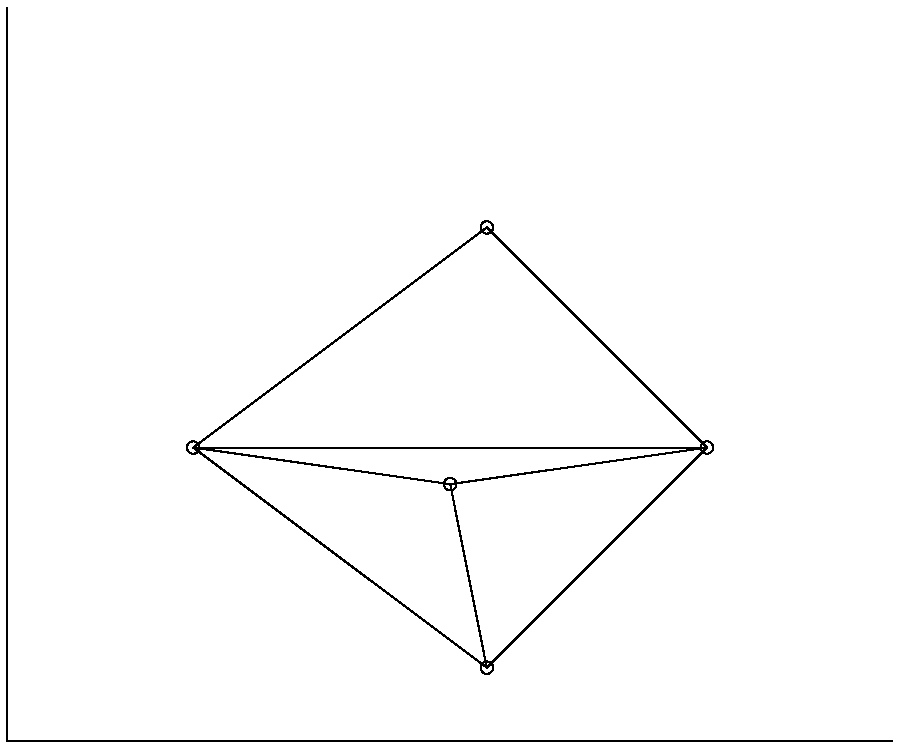
\includegraphics[width=0.4\columnwidth]{triangleplane-eps-converted-to.pdf}
\end{center}
\item The {\it Delaunay triangulation} is a special triangulation, often
considered optimal for interpolation purposes.
\end{itemize}
\end{frame}
\subsection{How is it useful?}
\begin{frame}{Uses}
\begin{itemize}
\item Mesh generation (e.g., for finite element methods)
\item Topological data analysis
\item Graph theory
\pause
\item \textbf{Piecewise linear multivariate interpolation}
\end{itemize}
\begin{center}
\includegraphics[width=0.4\columnwidth]{seamount-eps-converted-to.pdf}
\end{center}
\end{frame}

\begin{frame}{Interpolation}
\begin{itemize}
\item Let $T(P)$ be a $d$-dimensional triangulation of $P$.
\item Let $q \in CH(P)$ be an interpolation point, and let $S$ be a simplex
in $T(P)$ with vertices $s_1$, $\ldots$, $s_{d+1}$ such that $q\in S$.
\item Then there exist unique {\it convex weights} $w_1$, $\ldots$, $w_{d+1}$ 
such that $q = \sum_{i=1}^{d+1} w_i s_i$.
\end{itemize}
Define:
$$
\hat{f}_T (q) = f(s_1) w_1 + f(s_2) w_2 + \text{ $\ldots$ } + f(s_{d+1})w_{d+1}.
$$
\end{frame}

\section{Background}
\subsection{Formal Definition}
\begin{frame}{Definition of the Delaunay Triangulation}
The Delaunay triangulation is usually defined as the geometric dual of the
{\it Voronoi diagram}.
However, the following equivalent definition is preferred:
\begin{definition}
Let $C(v,r)$ denote a sphere of radius $r$ centered at $v$,
and let $B(v,r)$ denote the corresponding open ball: 
$$C(v,r):=\{x\in\mathbb{R}^d : \|x-v\|=r\}, \quad
B(v,r):=\{x\in\mathbb{R}^d:\|x-v\|<r\}.$$
A Delaunay triangulation $DT(P)$ of $n$ points $P \subset \mathbb{R}^d$ is any 
triangulation of $P$ such that for each
$d$-simplex $S\in DT(P)$, the $(d-1)$-sphere $C(v,r)$ circumscribing $S$
satisfies $B(v,r) \cap P = \emptyset$.
\end{definition}
\end{frame}
\begin{frame}{Visual of the Delaunay Triangulation}
A triangulation of 5 points in the plane $\mathbb{R}^2$ (left) and the
Delaunay triangulation of those same points (right):\\
\begin{center}
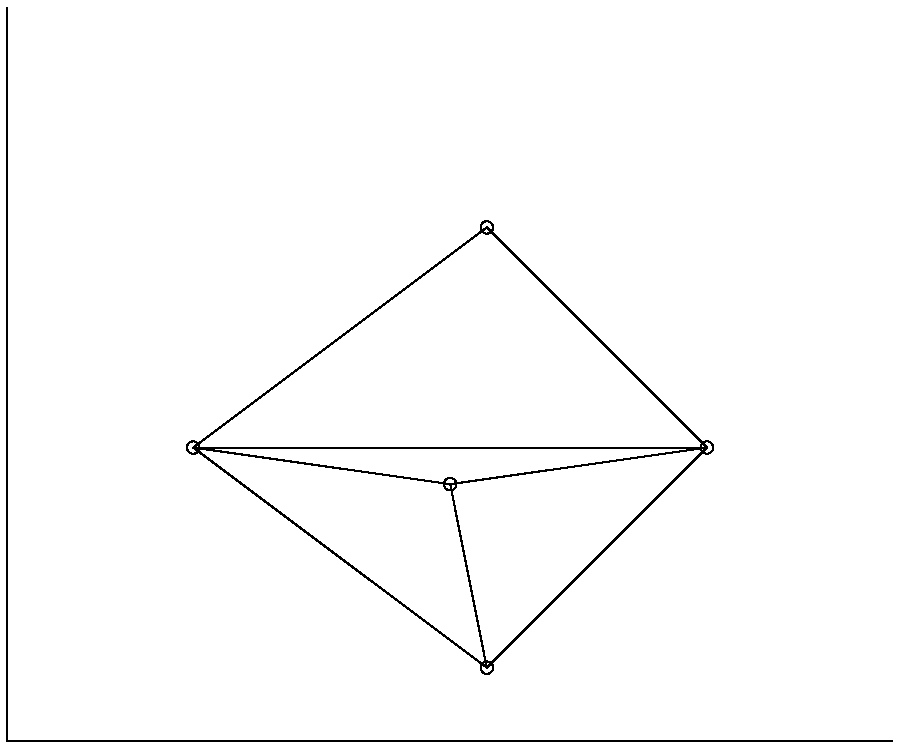
\includegraphics[width=0.4\columnwidth]{triangleplane-eps-converted-to.pdf}
\includegraphics[width=0.4\columnwidth]{delaunayplane-eps-converted-to.pdf}
\end{center}
\end{frame}
\begin{frame}{Existence and Uniqueness}
\begin{itemize}
\item Degeneracies:
\begin{itemize}
\item If all $n$ points in $P$ lie in some $(d-1)$-dimensional linear manifold,
then no triangulation can {\it exist}.
\item If $d+2$ or more points lie on the same $(d-1)$-sphere, then dividing
these $d+2$ points into $2$ or more $(d+1)$-simplices can be done arbitrarilly,
and the Delaunay triangulation is not {\it unique}.
\end{itemize}
\item If neither of the above 2 degeneracies occur, then the points are said
to be in {\it general position}, and the Delaunay triangulation $DT(P)$ exists
and is unique.
\end{itemize}
\end{frame}
\subsection{Challenges in High Dimensions}
\begin{frame}{Computability}
\begin{itemize}
\item There are many efficient algorithms for computing the two- and 
three-dimensional Delaunay triangulation (in $\mathbb{R}^2$ and $\mathbb{R}^3$)
generally running in $\mathcal{O}(n\log n)$ time.
\item However, in $\mathbb{R}^d$ the size of the Delaunay triangulation grows
exponentially! In the worst case: $\mathcal{O}(n^{\lceil\frac{d}{2}\rceil})$!\\
$\Rightarrow$
\begin{itemize}
\item Requires at least $\mathcal{O}(n^{\lceil\frac{d}{2}\rceil})$ time
to compute;
\item Requires at least $\mathcal{O}(n^{\lceil\frac{d}{2}\rceil})$ space
to store;
\end{itemize}
\end{itemize}
\pause
\begin{itemize}
\item :(
\end{itemize}
\end{frame}
\subsection{Previous Works}
\begin{frame}{Previous attempts!}
Many have tried to crack the curse of dimensionality!
\begin{itemize}
\item Bowyer-Watson (Bowyer and Watson 1981)
\item Quickhull (Barber, Dobkin, and Huhdanpaa, 1996)
\item CGAL --- Delaunay graph implementation
(Boissonnat, Devillers, and Hornus, 2009)
\end{itemize}
But ultimately, there's no getting around the exponential nature of the 
problem...
\end{frame}

\section{A New Algorithm}
\subsection{Addressing challenges}
\begin{frame}{A potential solution}

{\bf Proposed solution:} Instead of computing the whole triangulation, just 
compute the part we need!
\begin{itemize}
\item Recall the interpolation formula:
$$
\hat{f}_T (q) = f(s_1) w_1 + f(s_2) w_2 + \text{ $\ldots$ } + f(s_{d+1})w_{d+1}.
$$
Only dependent on a single simplex $S \in DT(P)$ (the simplex containing $q$)!
\item Can we compute $S$ without computing all of $DT(P)$?
\end{itemize}
\end{frame}
\subsection{Necessarry Operations}
\begin{frame}{Necessarry Operations}
There are three necessarry operations:
\pause
\begin{itemize}
\item Grow an initial simplex
\end{itemize}
\pause
\begin{itemize}
\item ``Flip'' a simplex
\end{itemize}
\pause
\begin{itemize}
\item Walk to containing simplex
\end{itemize}
\end{frame}
\begin{frame}{Growing Initial Simplex}
Minimize the radius of the initial circumsphere.
A greedy algorithm works!
\begin{itemize}
\item Pick initial point from $P$ arbitrarilly (closest point to $q$ is a 
good idea)
\item Pick second point from $P$ that is closest to $q$
\item Pick third point to minimize the radius of the smallest circumsphere
\item Etc...
\end{itemize}
\end{frame}
\begin{frame}{Flipping a Simplex}
Drop a point, then pick a new point on the ``other side'' of the remaining facet
to get a new simplex (hopefully ``closer'' to $q$)

\includegraphics[width=0.5\columnwidth]{circles-eps-converted-to.pdf}
\end{frame}
\begin{frame}{Simplex Walk}
Flip toward the next point using a ``visibility walk''
\begin{center}
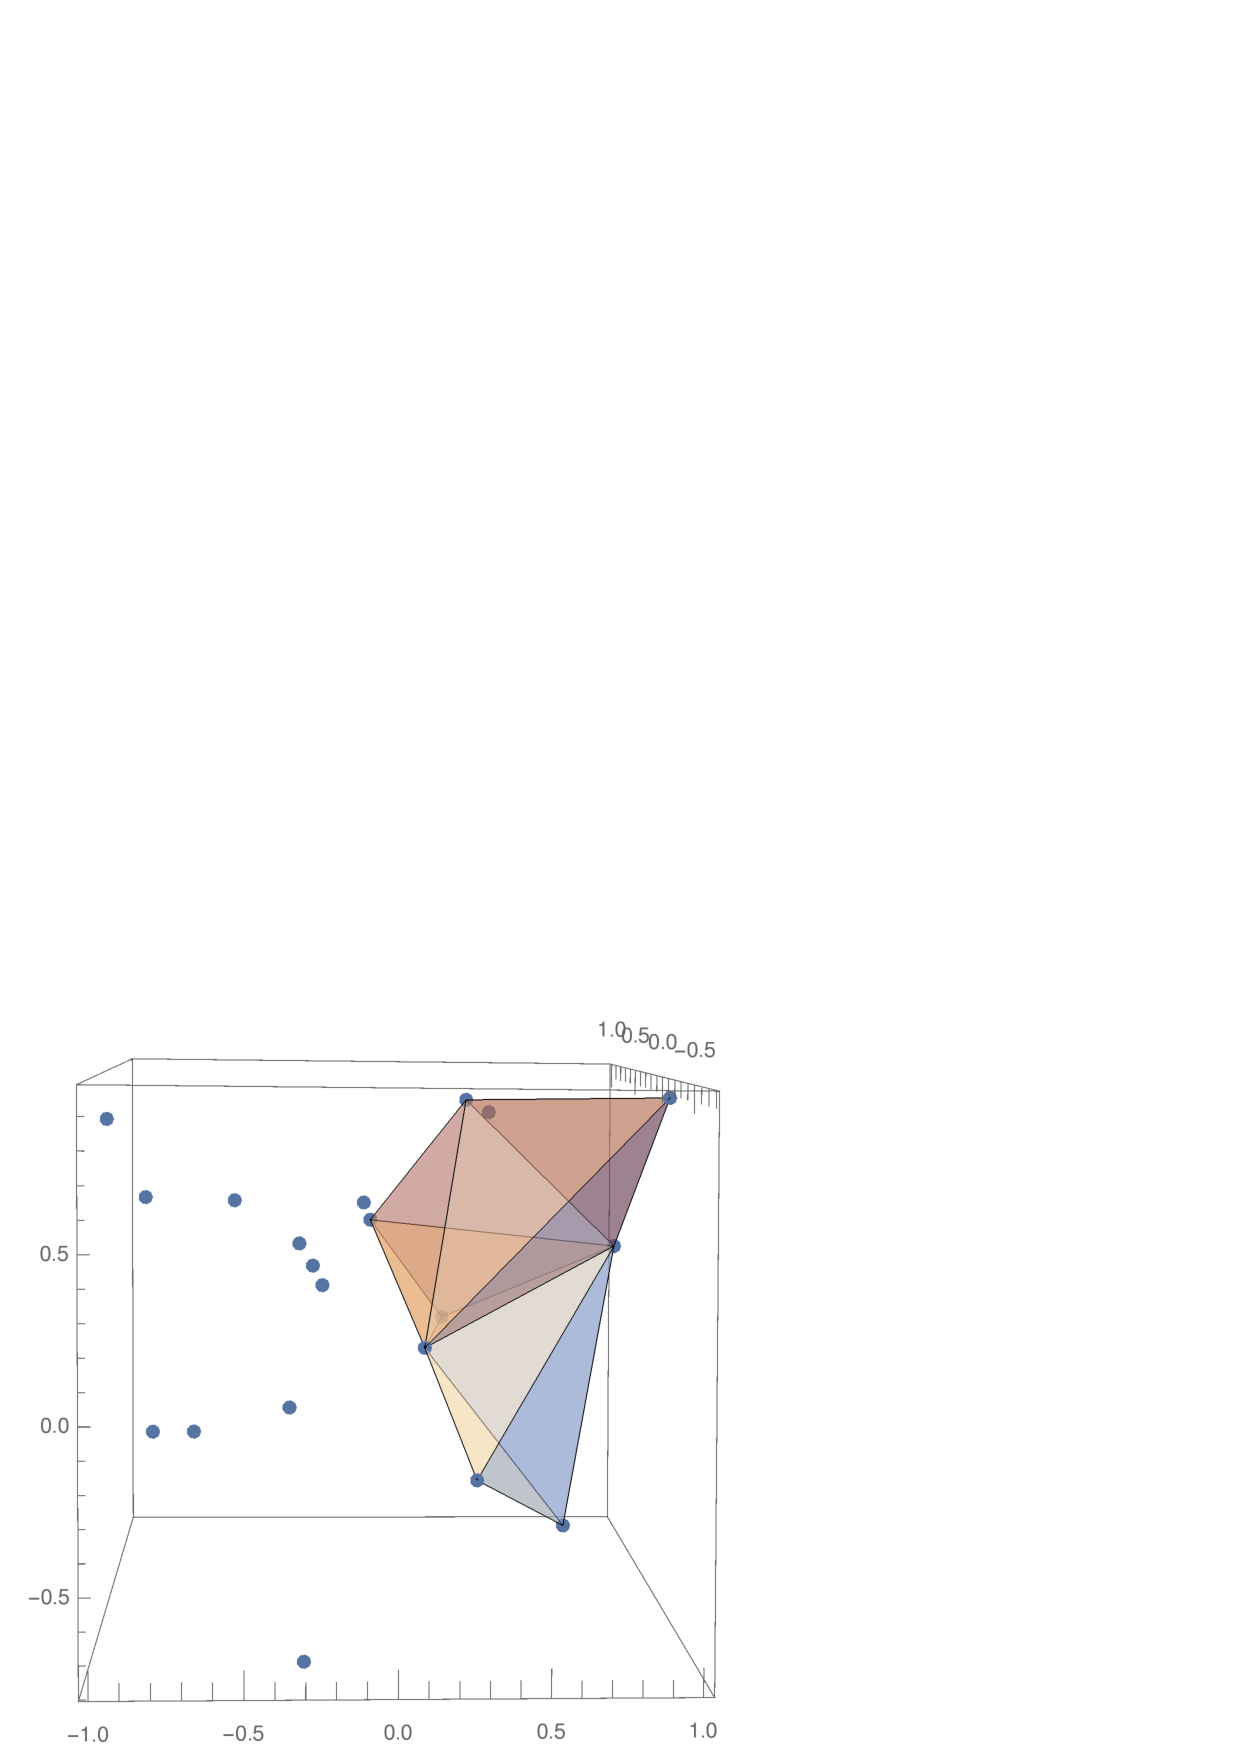
\includegraphics[width=0.5\columnwidth]{DelaunayWalk.pdf}
\end{center}
\end{frame}
\subsection{The New Algorithm}
\begin{frame}{The Algorithm}
\begin{itemize}
\item Grow an initial simplex
\item Flip ``toward'' $q$ using a visibility walk
\item Once we've found the simplex containing $q$, use the interpolation 
formula on the vertices of the simplex!
\end{itemize}
\end{frame}
\begin{frame}{Time/Space Complexity}
Total runtime:
\begin{itemize}
\item $\mathcal{O}(nd^4)$ to compute first simplex
\item $\mathcal{O}(nd^3)$ to compute each ``flip''
\item Total number of flips seems to be $\Theta(d\log d)$:
\end{itemize}
\begin{table}[htb]
\caption{Average number (with a sample size of 20) of Delaunay simplices 
computed in a simplex walk for $n$ pseudo-randomly generated points in 
$d$ dimensions.}
\label{tab:walk}
\centering
\begin{tabular}{l|cccc}
  & $n=2K$ & $n=8K$ & $n=16K$ & $n=32K$\\
\hline
$d=2$  & 3.05 & 2.90 & 3.25 & 3.10\\
$d=8$  & 23.75 & 24.75 & 24.30 & 23.10\\
$d=32$ & 95.25 & 125.60 & 131.85 & 150.10\\
$d=64$ & 171.95 & 221.85 & 248.35 & 280.60\\
\end{tabular}
\end{table}
\end{frame}
\begin{frame}{Issues in Stability}
\begin{itemize}
\item Points could all lie in a $(d-1)$-dimensional linear manifold
\begin{itemize}
\item Nothing to be done: Users should apply dimension reduction techniques
\end{itemize}
\item $d+2$ or more points lie in a $(d-1)$-sphere
\begin{itemize}
\item Delaunay triangulation still exists, but is not unique
\item Still, compute {\it a} Delaunay triangulation
\end{itemize}
\item A price to be paid! Extra computation time spent handling degeneracies.
\end{itemize}
\end{frame}

\section{Results and Conclusion}
\begin{frame}{Implementation}
\begin{itemize}
\item A serial numerically stable implementation of the proposed algorithm has
been coded in ISO Fortran 2003.
\item Tested for correctness against the standard implementation of Quickhull.
\item Runtimes gathered for pseudo-randomly generated data on a lab computer:
\item Note that Quickhull and other implementations don't scale past moderately
sized data sets in more than 5 or 6 dimensions, so there is no comparison.
\end{itemize}
\end{frame}
\begin{frame}{Results}
\begin{table}[htb]
\caption{Average runtime in seconds for interpolating at uniformly distributed
interpolation points for $n$ pseudo-randomly generated input points in 5
dimensions.}
\label{tab:uniform}
\centering
\begin{tabular}{r|cccc}
  & $n=2K$ & $n=8K$ & $n=16K$ & $n=32K$\\
\hline
32 interp. pts & 0.3 s & 2.7 s & 9.6 s & 35.7 s\\
1024 interp. pts & 2.5 s & 11.6 s & 28.9 s & 79.1 s\\
\end{tabular}
\end{table}
\end{frame}
\begin{frame}{Results}
\begin{table}[htb]
\caption{Average runtime in seconds for interpolating at clustered interpolation
points for $n$ pseudo-randomly generated input points in 5 dimensions.}
\label{tab:cluster}
\centering
\begin{tabular}{r|cccc}
  & $n=2K$ & $n=8K$ & $n=16K$ & $n=32K$\\
\hline
32 interp. pts & 0.2 s & 2.2 s & 8.4 s & 33.0 s\\
1024 interp. pts & 0.2 s & 2.5 s & 9.2 s & 35.2 s\\
\end{tabular}
\end{table}
\end{frame}
\begin{frame}{Results}
\begin{table}[htb]
\caption{Average runtime in seconds for interpolating at a single point
for $n$ pseudo-randomly generated input points in $d$-dimensional space .}
\label{tab:dimension}
\centering
\begin{tabular}{l|cccc}
  & $n=2K$ & $n=8K$ & $n=16K$ & $n=32K$\\
\hline
$d=2$ & 0.1 s & 1.7 s & 6.8 s & 27.0 s\\
$d=8$ & 0.2 s & 2.5 s & 9.6 s & 37.9 s\\
$d=32$ & 1.4 s & 9.5 s & 29.7 s & 101.1 s\\
$d=64$ & 13.2 s & 60.1 s & 138.6 s & 349.1 s\\
\end{tabular}
\end{table}
\end{frame}

\begin{frame}{Conclusion and Future Work}
\vfill
By taking advantage of the interpolation problem structure we are able to make 
this previously exponentially complex problem extremely scalable!
\vfill
In future work, these same techniques could be applied to other problems
that use Delaunay triangulations (including Voronoi diagrams).
\vfill
\end{frame}

\begin{frame}
\centering{{\Huge{QUESTIONS?}}}
\end{frame}

\end{document}
              
